\chapter{Grammar school}

\begin{quote}
``... small number
of symbols and their grammar are enough to capture the huge
variety of equations...''
\end{quote}

The point of a variable is to replace it.  So in the formula 
$x(x+3)^2$ replacing $x$ for $7$ gives us $7(7+3)^2$.  
Yet even in the land of algebra where every symbol is variable it is absurd to
replace $+$ for $7$ to get $x(x73)^2$.   There is restraint in the substitution
of algebra built into what makes something an algebraic formula. When we pull 
on this thread we unravel an expansive relationship between free algebras and induction
and their role in computation.

% It is none other than grammar.

Consider how we know what to do when   
calculating $7(7+3)^2$.  For some of us a mnemonic springs to mind
(\emph{Please Excuse My Dear Aunt Sally}) or an acronym (PEMDAS).
These both unwind to tell use Parenthesis Exponents Multiplication Division Addition Subtraction
in that order. This meandering thought process elucidates how we read formulas. 
The complexity 
can be visualized with a diagram called a \emph{parse tree}.
\begin{center}
    \begin{tikzpicture}
        \node (A) at (0,0) {\begin{tikzpicture}[yscale=0.75]
        \node (f) at (0,0) {$7(7+3)^2$};
        \node[below of=f,scale=0.75] {$\times$};
        \node (x1) at (-1,-2) {$7$};
        \node (sqrt1) at (1,-2) {$(7+3)^{2}$}; 
        % \node[below of=sqrt1,scale=0.75] {$\circ$};
        \node (su) at (1.5,-3) {\textasciicircum $2$};
        \node (u) at (1,-4) {$7+3$};
        \node (x2) at (0,-6) {$7$};
        \node[below of=u,scale=0.75] {$+$};
        \node (three) at (2,-6) {$3$};
        % \node (x3) at (0,-8) {$x$};
        % \node (x4) at (2,-8) {$x$};
        % \node[below of=x2,scale=0.75] {$\times$};

        \draw[-] (f) -- (x1);
        \draw[-] (f) -- (sqrt1);
        % \draw[-] (sqrt1) -- (su);
        \draw[-] (sqrt1) -- (u);
        \draw[-] (u) -- (x2);
        \draw[-] (u) -- (three);
        % \draw[-] (x2) -- (x3);
        % \draw[-] (x2) -- (x4);

    \end{tikzpicture}};
    
    \node[right of=A,xshift=3cm] (B) {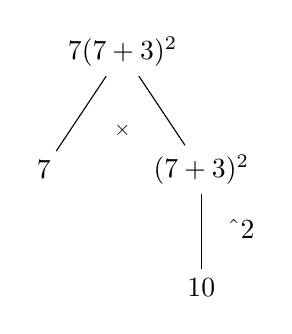
\begin{tikzpicture}[yscale=0.75]
        \node (f) at (0,0) {$7(7+3)^2$};
        \node[below of=f,scale=0.75] {$\times$};
        \node (x1) at (-1,-2) {$7$};
        \node (sqrt1) at (1,-2) {$(7+3)^{2}$}; 
        % \node[below of=sqrt1,scale=0.75] {$\circ$};
        \node (su) at (1.5,-3) {\textasciicircum $2$};
        \node (u) at (1,-4) {$10$};

        \draw[-] (f) -- (x1);
        \draw[-] (f) -- (sqrt1);
        % \draw[-] (sqrt1) -- (su);
        \draw[-] (sqrt1) -- (u);

    \end{tikzpicture}};
    
    \node[right of=B, xshift=3cm] (C) {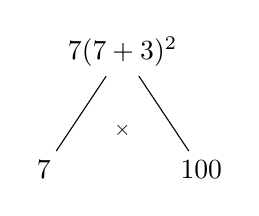
\begin{tikzpicture}[yscale=0.75]
        \node (f) at (0,0) {$7(7+3)^2$};
        \node[below of=f,scale=0.75] {$\times$};
        \node (x1) at (-1,-2) {$7$};
        \node (sqrt1) at (1,-2) {$100$}; 

        \draw[-] (f) -- (x1);
        \draw[-] (f) -- (sqrt1);

    \end{tikzpicture}};
    \node[right of=C,xshift=1cm] {$700$};

    \draw[thick] (A.north east) -- (A.south east);
    \draw[thick] (B.north east) -- (B.south east);
    \draw[thick] (C.north east) -- (C.south east);
\end{tikzpicture}
\end{center}
We can read the tree like step-by-step instructions. Above and 
throughout this book we use the comic-strip method to separate diagrams 
evolving over time, reading time as left-to-right top-to-bottom.  Start at the leaves and join
them by whatever operation is displayed on adjacent branches.
We start at the bottom with $7,3$, and join them as $7+3$ (computing $10$),
then the next step is to square (now $100$), then multiply by $7$, we reach $700$.
In hindsight, we taught children a complicated form of induction.

You may have been taught induction through stories of falling 
dominos.  Good.  But what if induction was more like what we just did, climbing?
The domino illustration could bottle up the experience of climbing stairs.  
Now we climb trees and maybe mountains.
Setting up this induction was nothing more than a fragment of text but 
read through the lens of a grammar, e.g.\ PEMDAS, it came into a full form
as steps for recursion.

Climbing could find many routes, even go in cycles, but 
evaluating a formula was a precise algorithm without ambiguity.
The reason was that we had a tree.  Trees have unique paths between 
any two vertices. So if we start at the bottom we have a unique direction to 
reach the top.  Recursion on trees is so special it has a special name:
\emph{traversing} the tree.  

Parsing grammars in natural language is not always that
uniform.  A simplistic English grammar will often parse into cycles.
\begin{center}
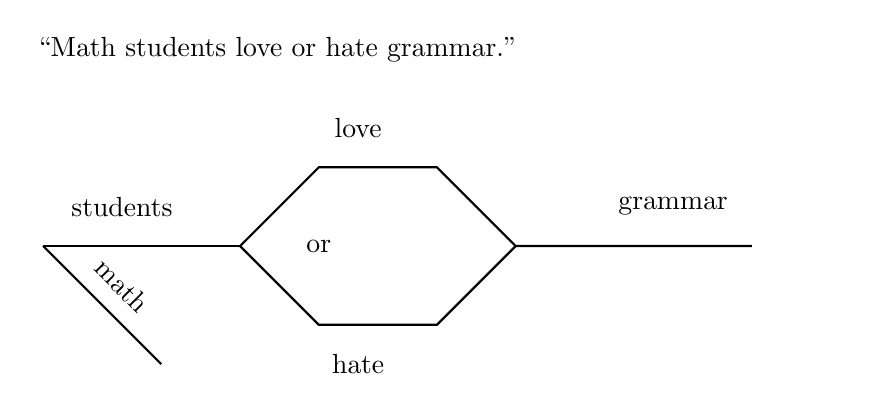
\begin{tikzpicture}
    \node[text width=4in] at (1,2) {``Math students love or hate grammar.''};
    \node at (-3,0) {students};
    \node[rotate=-45] at (-3,-1) {math};
    \node at (-0.5,-0.5) {or};
    \node at (0,1) {love};
    \node at (0,-2) {hate};
    \node at (4,0) {grammar};

    \draw[thick] (-4,-0.5) -- ++(2.5,0);
    \draw[thick] (-4,-0.5) -- ++(1.5,-1.5);
    \draw[thick] (-1.5,-0.5) -- ++(1,1) -- ++(1.5,0) -- ++(1,-1) -- ++(3,0);
    \draw[thick] (-1.5,-0.5) -- ++(1,-1) -- ++(1.5,0) -- ++(1,1);

\end{tikzpicture}
\end{center}
In mathematics two paths to the same place are said to be a relation, 
they are related.  So systems that have no cycles, i.e.\ trees, are 
free of relations, or simply \emph{free}.  In time we will come to see 
that every algebraic structure can be constructed from a free 
structure with the possible addition of relations.

\begin{remark}
    Having two formulas that reduce to the same value is not the same 
as a relation in the grammar.  So what is free in this case 
is the grammar we used for arithmetic formulas.  
For example $7(7+3)(7+3)$ renders the same result 700, and nearly 
by the same steps.  Yet, if we diagrammed that formula as a
parse tree it would quite different
\begin{center}
    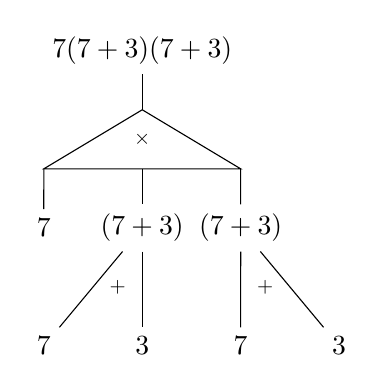
\begin{tikzpicture}[xscale=1.25,yscale=0.75]
        \node (t) at (0,1) {$7(7+3)(7+3)$};
        \node (a) at (-1,-2) {$7$};
        \node (b) at (0,-2) {$(7+3)$}; 
        \node (c) at (1,-2) {$(7+3)$};
        \node (e) at (-1,-4) {$7$};
        \node (f) at ( 0,-4) {$3$};
        \node (g) at ( 1,-4) {$7$};
        \node (h) at ( 2,-4) {$3$};

        \draw (0,0) -- (-1,-1) -- (1,-1) -- cycle;

        \node[scale=0.75] at (0,-0.5) {$\times$};
        \node[scale=0.75] at (-0.25,-3) {$+$};
        \node[scale=0.75] at ( 1.25,-3) {$+$};

        \draw[-] (t) -- (0,0);
        \draw[-] (-1,-1) -- (a);
        \draw[-] (0,-1) -- (b);
        \draw[-] (1,-1) -- (c);
        \draw[-] (b) -- (e);
        \draw[-] (b) -- (f);
        \draw[-] (c) -- (g);
        \draw[-] (c) -- (h);
    \end{tikzpicture}    
\end{center}    
In particular we have not even expressed this as a pair of products 
we have asked instead for a function that takes products of three 
numbers at once.  The ambiguity of how we might achieve this is hidden in the 
triangle \emph{operad} labeled $\times$.
\end{remark}

\index{context-free}
That we got a tree in math formulas means we have a rather boring grammar, 
what Chompsky's \emph{Syntactic Structure} calls
\emph{context-free} grammars.\footnote{
    If an algebraist starts a talk with a story that ``...It was thought  all natural 
    languages were context-free until some obscure dialect in the alps or Africa was found...'', 
    then tune out until they return to equations.  
    Linguist never had such illusions. Even english is not context-free, read  James Higginbotham.} 
Don't be too disheartened.  Virtually every programming language has a 
context-free grammar and programs can communicate a lot of hefty ideas. 

\begin{quote}
    \textbf{Complex inductions can be specified by grammar.}
\end{quote}
